\documentclass[a4paper,11pt]{article}

% Use utf-8 encoding for foreign characters
\usepackage[utf8]{inputenc}
\usepackage[british,english]{babel}
\usepackage[T1]{fontenc}

% Setup for fullpage use
\usepackage{fullpage}

% Multipart figures
\usepackage{subfigure}

% More symbols
\usepackage{amsmath}
\usepackage{amssymb}
\usepackage{latexsym}

\usepackage{booktabs}

% For pretty URLs, see: http://en.wikibooks.org/wiki/LaTeX/Hyperlinks
\usepackage{hyperref}

% Surround parts of graphics with box
\usepackage{boxedminipage}

% Package for including code in the document
\usepackage{listings}

% If you want to generate a toc for each chapter (use with book)
\usepackage{minitoc}

% Uncomment if you want to use Palatino as font
\usepackage[sc]{mathpazo}
\linespread{1.05}         % Palatino needs more leading (space between lines)

% This is now the recommended way for checking for PDFLaTeX:
\usepackage{ifpdf}

% Used for highlighting text with \hl{}
\usepackage{soul}

\addto\captionsenglish{\renewcommand{\refname}{}}

%\newif\ifpdf
%\ifx\pdfoutput\undefined
%\pdffalse % we are not running PDFLaTeX
%\else
%\pdfoutput=1 % we are running PDFLaTeX
%\pdftrue
%\fi

\ifpdf
\usepackage[pdftex]{graphicx}
\else
\usepackage{graphicx}
\fi
\title{Deliverable 6: Sprint \#4\\\small{for}\\\small{Danske Bank: Peer-to-peer}}
\author{ Group Delta:\\Jesper Borgstrup, Thomas Kjeldsen and Mads Ohm Larsen }

\date{May 20, 2011}

\begin{document}

\ifpdf
\DeclareGraphicsExtensions{.pdf, .jpg, .tif}
\else
\DeclareGraphicsExtensions{.eps, .jpg}
\fi

\maketitle

%\tableofcontents
%\vspace{2cm}

%%%%%%%%%%%%%%%%%%%%%%%%%%%%%%%%%%%%%%
%%%%%%%%%%%%%%%%%%%%%%%%%%%%%%%%%%%%%%
%%%%%%%%%%%%%%%%%%%%%%%%%%%%%%%%%%%%%%

\section{Requirements for this deliverable}
\begin{enumerate}
\item Doing a demo in class (on 2011-05-18)
\item Giving us access to your source code
\item Handing in a collection of your sprint material
\item Describing a sprint retrospective (e.g., as a set of bullets outlining what
when well, what went wrong, and how you will improve for the next sprint)
\end{enumerate}

The Sprint Demo was given on May 18th. This document describes requirements 2-4 as well as the sprint learning goal -- mutual code inspection in our group and group Bravo.

%%%%%%%%%%%%%%%%%%%%%%%%%%%%%%%%%%%%%%
%%%%%%%%%%%%%%%%%%%%%%%%%%%%%%%%%%%%%%
%%%%%%%%%%%%%%%%%%%%%%%%%%%%%%%%%%%%%%

\section{Inspection}
Our group was set to do code inspection of parts of the code from group Bravo, as well as they were set to do inspection of our code. This section covers the results of their inspection of our code.

We asked the group to inspect the following files from the commit \href{https://github.com/omegahm/DBP2P/commit/5a08a6a2c3a4d11663ae10a8ee2b371f69f2eab9}{5a08a6a2...eab9} in the folder {\tt src/dk/hotmovinglobster/dustytyba}:

\begin{itemize}
\item {\tt api/BTAPI.java}
\item {\tt api/BTAPIListener.java}
\item {\tt api/BtConnection.java}
\item {\tt id/GenericIPActivity.java}
\item {\tt id/ManualIPActivity.java}
\end{itemize}

The results of the inspection are shown in table \ref{inspection-results} with Fagan (1976) error format (type/cause/severity). The three types are:

\begin{description}
\item{PR} Programming anomaly
\item{LO} Logic
\item{CO} Comment
\end{description}

\begin{table}
\begin{tabular}{llrl}
\toprule
\ \  & {\bf Type} & {\bf Line(s)} & {\bf Description} \\
\midrule
\multicolumn{4}{l}{{\bf {\tt api/BtAPIListener.java}}} \\
& {\tt PR/W/MIN} & 9 & The interface need not be abstract? \\
\midrule
\multicolumn{4}{l}{{\bf {\tt api/BtAPI.java}}} \\
& {\tt LO/M/MIN} & N/A & Static variables are not only defined in the top \\
\midrule
\multicolumn{4}{l}{{\bf {\tt api/BTConnection.java}}} \\
& {\tt LO/W/MAJ} & 28-34 & Getters and setters are bad for static variables \\
& {\tt CO/W/MIN} & 38 & The comment says "for internal use", but the constructor is public \\
& {\tt LO/M/MIN} & 51 & Missing catch of IOException \\
& {\tt LO/E/MIN} & 104 & diconnect() does nothing \\
& {\tt PR/W/MIN} & 111 & Magic constant 1024 for buffer \\
\bottomrule
\end{tabular}
\caption{Results of the code inspection from group Bravo. Note that nothing were to report on code on in the {\tt id} folder.}
\label{inspection-results}
\end{table}


%%%%%%%%%%%%%%%%%%%%%%%%%%%%%%%%%%%%%%
%%%%%%%%%%%%%%%%%%%%%%%%%%%%%%%%%%%%%%
%%%%%%%%%%%%%%%%%%%%%%%%%%%%%%%%%%%%%%

\section{Source code access}
Our source code is publicly available on GitHub from \url{https://github.com/omegahm/DBP2P}.

If you wish to checkout our code (read-only) using Git, then use git clone with this URL:
\url{git://github.com/omegahm/DBP2P.git}

The presentation given in class with the instructions and code to get the library working can be found on this URL:

\noindent \url{https://docs.google.com/present/edit?id=0AVZYqiAJzRZpZGN3YzhoazNfMjZnYjRzOWtnYw&hl=da&authkey=CMO8gOYD}.

{ % TODO
\texttt{\hl{REPLACE WITH CURRENT REPO URL}\\}
}

%%%%%%%%%%%%%%%%%%%%%%%%%%%%%%%%%%%%%%
%%%%%%%%%%%%%%%%%%%%%%%%%%%%%%%%%%%%%%
%%%%%%%%%%%%%%%%%%%%%%%%%%%%%%%%%%%%%%

\section{Sprint material}
Sprint Material needed to assess our progress include the following:
\begin{itemize}
\item source code (version number and access method is sufficient)
\item product backlog (before and after the sprint)
\item sprint backlog
\item any other material (e.g., burndown chart) that illustrates your progress
\end{itemize}


%The final product of sprint \#4 has been tagged \href{https://github.com/omegahm/DBP2P/tree/sprintdemo2}{\tt sprintdemo3}. in the git repository, where the application is located in the folder {\tt DustyTubaSampleApp}.

%The following main tasks have been completed during this sprint:
%\begin{itemize}
%	\item ``Libraryfying'' our code
%	\item Using the library to establish Bluetooth connection (2.1+ devices only)
%	\item Wrote documentation
%	\begin{enumerate}
%		\item Both for future developers of the library, as well as for users of the library
%	\end{enumerate}
%\end{itemize}

In regards to our user stories, the tasks completed correspond to the following user story:
\begin{verbatim}
  As a        user
  I want to   be able to see a list of friends
  Such that   I can quickly find people I often send items to
\end{verbatim}

\subsection{Sprint Backlog}
Our sprint backlog is shown in figure \ref{sprintbacklog} on page \pageref{sprintbacklog}.

{ % TODO
\texttt{\hl{REPLACE WITH CURRENT PICTURE}}
}

 \begin{figure}[ht!]
	\begin{center}
 	% Insert sprint backlog here
 	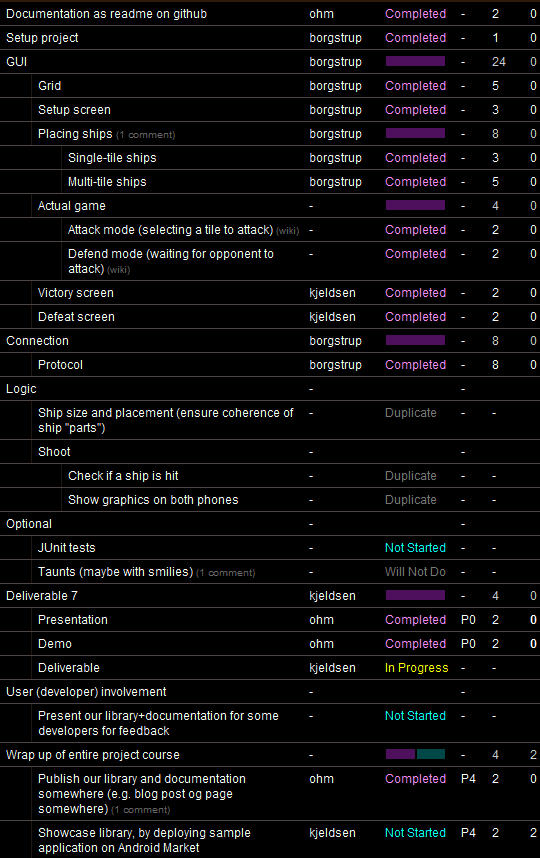
\includegraphics[width=0.85\textwidth]{sprint_backlog.png}		
 	\end{center}
 	\caption{Our sprint backlog after the sprint was finished}
 	\label{sprintbacklog}
 \end{figure}

\subsection{Burndown chart}

Our burndown chart is shown in figure \ref{burndown} on page \pageref{burndown}.

{ % TODO
\texttt{\hl{REPLACE WITH CURRENT PICTURE}\\}
}

 \begin{figure}[ht!]
 	\begin{center}
 	% Insert burndown chart here
 	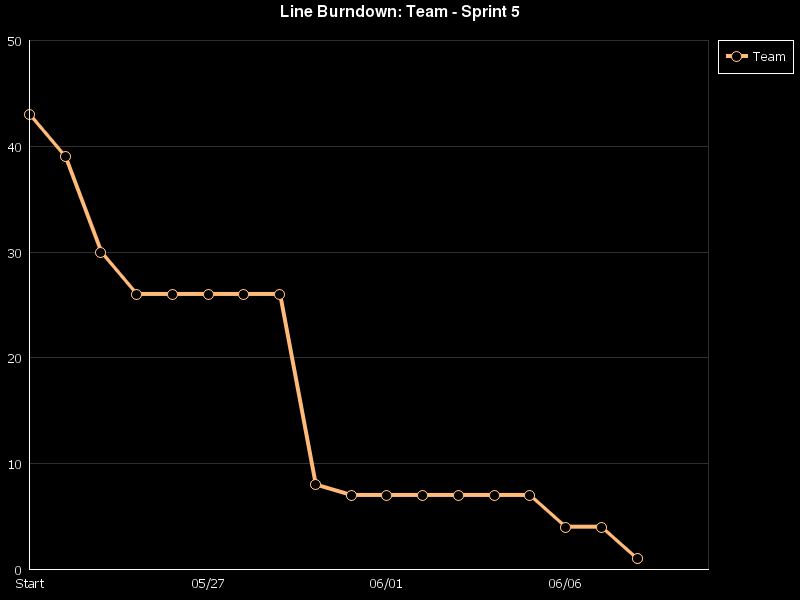
\includegraphics[width=\textwidth]{line_burndown.png}		
 	\end{center}
 	\caption{Our burndown chart at the end of the sprint}
 	\label{burndown}
 \end{figure}

%\subsection{Acunote}
%We have got an Acunote account\footnote{\url{http://dbp2p.acunote.com/}} setup, and %access to this have been granted.
%
%\clearpage
%
%%%%%%%%%%%%%%%%%%%%%%%%%%%%%%%%%%%%%%
%%%%%%%%%%%%%%%%%%%%%%%%%%%%%%%%%%%%%%
%%%%%%%%%%%%%%%%%%%%%%%%%%%%%%%%%%%%%%

\clearpage

\section{Sprint retrospective}

What went well during this sprint:

\begin{itemize}
%\item Great success w/ presentation despite laziness and unpreparedness
\item Good estimation of workload
\item Good division of tasks between team members
\end{itemize}

\noindent
What went wrong:
\begin{itemize}
%\item Pairing of phones, since we didn’t start from scratch (or pre-pair phones)
%\item Slow demo PC
\item Original sprint goal wasn’t feasible, so we had to redefine goal in-sprint.
\item We didn’t check in to acunote as often as desirable
\end{itemize}

\noindent
How we will improve:
\begin{itemize}
\item The last sprint goal will be feasible
\item We will check in to acunote more often
\end{itemize}

\end{document}
